% File: chapters/implementation.tex

\chapter{Implementation}
\label{chap:implementation}

We turned the methodology from Chapter 3 into working code and systems over the course of this implementation. The three research phases defined in Chapter~3 (Section~\ref{sec:meth_strategy}), namely Phase~1: Local LLM Evaluation (Section~\ref{sec:impl_phase1}), Phase~2: Model Optimization with LoRA (Section~\ref{sec:impl_phase2}), and Phase~3: Enterprise CI/CD Integration (Section~\ref{sec:impl_phase3}), map directly to the development progression described below. Each phase built on the previous one. The following sections cover our tool choices, the specific steps we followed, and the engineering decisions we made along the way.

\section{Toolchain Selection and Rationale}
\label{sec:impl_toolchain}

Before writing any code, we needed to select the appropriate tools. Several factors guided the selection. Research reproducibility required tools with stable APIs and clear documentation. Industrial deployment required compatibility with CARIAD's existing infrastructure. Hardware specifications influenced which models could run locally with acceptable performance.

\subsection{Fuzzing Infrastructure}

For the fuzzing engine itself, we chose libFuzzer combined with Clang sanitizers. libFuzzer is the industry standard for coverage-guided fuzzing in C and C++ projects \cite{LibFuzzer2015}, though alternatives like AFL++ \cite{AFLPlusPlus} also have strong communities. libFuzzer integrates directly with the LLVM toolchain, which means compilation and fuzzing use the same infrastructure. Google uses libFuzzer for OSS-Fuzz \cite{OSSFuzzBugs2021}, so the documentation and community support are excellent.

We compiled all targets with AddressSanitizer (ASan) and UndefinedBehaviorSanitizer (UBSan) enabled. ASan catches memory errors like buffer overflows, use-after-free, and memory leaks \cite{LibFuzzer2015}. UBSan catches undefined behavior like signed integer overflow and null pointer dereferences. These sanitizers add runtime overhead, but for security testing the tradeoff is acceptable, since detecting vulnerabilities takes priority over execution speed.

For integration with our build systems, we used cifuzz from Code Intelligence. The tool wraps libFuzzer and provides additional functionality like corpus management, coverage reporting, and build system integration. The most relevant feature for our work was cifuzz spark, which handles the LLM integration. Spark takes a CMake target as input, extracts API information automatically, sends it to the configured LLM, and produces a fuzz driver ready for execution.

Our choice of cifuzz was based on a systematic evaluation. We compared several alternatives including Google's ClusterFuzz \cite{OSSFuzzBugs2021} and standalone libFuzzer setups. Among these, cifuzz offered a good balance between ease of use and enterprise features. Its spark module specifically addressed our core research question by providing a clean interface between the fuzzing infrastructure and LLM backends.

\subsection{LLM Infrastructure}

We needed to run models locally for several reasons. First, evaluating many different models through paid APIs would have been cost-prohibitive. Second, some models are open-source and only available for local deployment. Third, understanding local deployment options was essential for the enterprise integration phase.

We selected Ollama \cite{ollama} as our primary local inference server. Ollama simplifies model management. Installing a new model is one command: \texttt{ollama pull qwen2.5-coder:32b}. The server exposes an OpenAI-compatible API, which meant cifuzz spark worked without modification. Ollama handled quantized models well. Quantization compresses models to use reduced numerical precision (e.g., 4-bit instead of 16-bit weights), which let us run larger models on the available hardware.

For models not available through Ollama, we used llama.cpp directly. This required more manual configuration but provided additional flexibility. Some models from Hugging Face came as split GGUF files that needed merging before use. We handled this with the following command:

\begin{lstlisting}[language=bash, caption={Merging Split GGUF Model Files}]
llama-gguf-split --merge qwen2.5-coder-14b-instruct-q5_k_m-00001-of-00002.gguf \
                 qwen2.5-coder-14b-instruct-q5_k_m.gguf
\end{lstlisting}

Merging these split files added an extra step to our model preparation process.

For cloud deployment in the enterprise phase, we configured Azure OpenAI \cite{azure_openai}. Azure provided GPT-4o through a managed endpoint. The authentication used API keys stored as GitHub secrets. We configured the following environment variables:

\begin{lstlisting}[language=bash, caption={Azure OpenAI Configuration}]
export CIFUZZ_LLM_API_URL="https://ny4mdomain.openai.azure.com"
export CIFUZZ_LLM_AZURE_DEPLOYMENT_NAME="gpt-4o"
export CIFUZZ_LLM_API_TOKEN="<api-key>"
export CIFUZZ_LLM_MAX_TOKENS=40000
\end{lstlisting}

A token limit of 40,000 was necessary because fuzz driver generation requires extensive context. A typical prompt includes the extracted API context (header files with function signatures), fuzzing instructions (libFuzzer entry-point requirements, safety constraints), and optionally example driver snippets. Smaller token limits led to truncation and reduced output quality. A representative example prompt is provided in Appendix~\ref{sec:appendix_prompt}.

\subsection{Development Environment}

Local development happened on a MacBook Pro with an M1 Pro chip. For Linux container support on Apple Silicon, we chose Podman as our container runtime. Podman aligned well with the enterprise CI/CD runners, which also used Linux.

\begin{lstlisting}[language=bash, caption={Podman Setup on macOS}]
brew install podman
podman machine init --cpus 4 --memory 8192
podman machine start
\end{lstlisting}

Transitioning from Docker to Podman involved adapting several scripts to align with Podman's container networking model.

For the enterprise environment, we used CARIAD's internal GitHub Enterprise instance with self-hosted runners. These runners used Buildah \cite{buildah} instead of Docker for container operations. Buildah is daemonless, which complies with security policies that govern long-running daemon processes.

Our build toolchain used CMake for project configuration and Clang for compilation. We required CMake version 3.5 or higher because cifuzz integration depends on features from that version. The CMake configuration for enabling fuzzing required minimal setup:

\begin{lstlisting}[language=cmake, caption={CMake Fuzzing Configuration}]
cmake_minimum_required(VERSION 3.5)
cmake_policy(VERSION 3.5)

project(FuzzTarget)

find_package(cifuzz NO_SYSTEM_ENVIRONMENT_PATH)
enable_fuzz_testing()
add_subdirectory(cifuzz-spark)
\end{lstlisting}

We also needed to update CMakeLists.txt files in subdirectories. Several target libraries used CMake configurations that needed updates for compatibility with our setup. The fix was consistent across all subdirectories:

\begin{lstlisting}[language=cmake, caption={Subdirectory CMake Updates}]
cmake_minimum_required(VERSION 3.10...3.22)
cmake_policy(VERSION 3.10...3.22)
\end{lstlisting}

The LLM-assisted fuzzing workflow, conceptually introduced in Chapter~3, demonstrates how LLMs integrate into the fuzzing pipeline to automatically generate test cases from source code. Our implementation uses cifuzz spark to handle the integration between the LLM backends (either local models via Ollama or Azure OpenAI) and the libFuzzer execution environment.

\section{Phase 1: Local LLM Evaluation Setup}
\label{sec:impl_phase1}

Phase 1 focused on understanding which models could generate useful fuzz drivers. The experiments in this phase target \textbf{RQ1} (Can LLMs generate compilable, executable fuzz drivers?) and \textbf{RQ2} (Does model size determine quality?). We did not assume any model would work well. Literature suggested mixed results for LLM code generation, and fuzz drivers are a specialized task.

\subsection{Benchmarked Models}

We evaluated 14 models spanning a wide range of sizes and architectures. The selection included both general-purpose models and code-specialized variants. Our goal was to understand whether model size, training data, or architecture had the greatest impact on fuzz driver quality.

\textbf{Large Models (25 to 35 billion parameters):}
\begin{itemize}
    \item Qwen 2.5-Coder 32B
    \item DeepSeek Coder 33B
    \item CodeLlama 34B Instruct
    \item WizardCoder 34B
    \item Yi 34B
    \item Gemma 3 27B
\end{itemize}

\textbf{Extra Large Models (above 40 billion parameters):}
\begin{itemize}
    \item Mixtral 46.7B (Mixture-of-Experts architecture, approximately 12.9B active parameters per inference)
\end{itemize}

\textbf{Medium Models (7 to 16 billion parameters):}
\begin{itemize}
    \item Qwen 2.5-Coder 7B and 14B
    \item Phi-4 14B
    \item DeepSeek Coder V2 Lite 16B
    \item Gemma 3 9B
\end{itemize}

\textbf{Small Models (below 7 billion parameters):}
\begin{itemize}
    \item Qwen 2.5-Coder 1.5B
    \item Gemma 3 4B
\end{itemize}

Code-specialized models like Qwen Coder, DeepSeek Coder, and CodeLlama were trained specifically on programming tasks. General-purpose models like Mixtral, Yi, Gemma~3, and Phi-4 were included to investigate whether broad training with strong code exposure could compensate for lack of explicit code specialization. This allowed us to test a key hypothesis, whether a 46B general model outperforms a 7B code-specialized model. Results, discussed in Chapter~5, were surprising: the general-purpose Yi (34B) achieved 0\% code coverage at runtime, and Mixtral (46.7B) could not be evaluated at all due to hardware constraints, while Qwen 2.5-Coder (32B) and Gemma 3 (27B) consistently achieved over 43\% line coverage. Even some code-specialized models like CodeLlama (34B) did not produce working drivers, suggesting that neither code specialization nor model size alone is sufficient without adequate training on relevant code patterns.

Installing these models required considerable disk space. The larger models exceeded 20~GB each in their quantized forms. We used 4-bit and 5-bit quantization to fit models into available VRAM while maintaining reasonable output quality. A complete summary of all 14 evaluated models, including their parameter counts, quantization levels, architectures, and results, is provided in Table~\ref{tab:impl_model_summary} and in the appendix (Table~\ref{tab:appendix_all_models}).

\begin{table}[htbp]
\centering
\caption{Summary of All Evaluated Models on yaml-cpp}
\label{tab:impl_model_summary}
\resizebox{\textwidth}{!}{%
\begin{tabular}{llccccl}
\toprule
Model & Type & Params & Quant. & Disk Size & yaml-cpp Cov. & Status \\
\midrule
Qwen 2.5-Coder 32B & Code-specialized & 32B & Q4\_K\_M & $\sim$20\,GB & 43.08\% & Functional \\
Gemma 3 27B & General-purpose & 27B & Q4\_K\_M & $\sim$17\,GB & 45.06\% & Functional \\
Phi-4 14B & General-purpose & 14B & Q4\_K\_M & $\sim$9\,GB & 34.26\% & Functional \\
Qwen 2.5-Coder 14B & Code-specialized & 14B & Q5\_K\_M & $\sim$10\,GB & 0\% & Compile failure \\
Qwen 2.5-Coder 7B & Code-specialized & 7B & Q5\_K\_M & $\sim$5\,GB & 0\% & Compile failure \\
Qwen 2.5-Coder 1.5B & Code-specialized & 1.5B & FP16 & $\sim$3\,GB & 0\% & Compile failure \\
DeepSeek Coder 33B & Code-specialized & 33B & Q4\_K\_M & $\sim$20\,GB & 0\% & Compile failure \\
DeepSeek Coder V2 Lite & Code-specialized (MoE) & 16B & Q4\_K\_M & $\sim$10\,GB & 0\% & Compile failure \\
CodeLlama 34B Instruct & Code-specialized & 34B & Q4\_K\_M & $\sim$20\,GB & 0\% & Compile failure \\
WizardCoder 34B & Code-specialized & 34B & Q4\_K\_M & $\sim$20\,GB & 0\% & Compile failure \\
Yi 34B & General-purpose & 34B & Q4\_K\_M & $\sim$20\,GB & 0\% & Invalid API usage \\
Gemma 3 9B & General-purpose & 9B & Q4\_K\_M & $\sim$6\,GB & 0\% & Compile failure \\
Gemma 3 4B & General-purpose & 4B & Q4\_K\_M & $\sim$3\,GB & 0\% & Compile failure \\
Mixtral 46.7B & General-purpose (MoE) & 46.7B & Q4\_K\_M & $\sim$28\,GB & N/A & Hardware limit \\
\bottomrule
\end{tabular}%
}
\end{table}

\subsection{Target Repositories}

Consistent test targets were needed for fair model comparison. Our selection included open-source C++ libraries with varying complexity:

\textbf{Primary Target: yaml-cpp}

yaml-cpp is a YAML parsing library with approximately 35 source files and over 1000 API candidates that could potentially be fuzzed. We chose it as our primary benchmark because it has enough complexity to challenge the models while being well documented and actively maintained. The library also has existing fuzz targets in OSS-Fuzz, giving us a baseline for comparison.

\textbf{Secondary Targets:}
\begin{itemize}
    \item \textbf{RapidJSON}: A JSON parsing library widely used in performance-critical applications. RapidJSON's CMake configuration needed adjustments for our setup, which we resolved by re-downloading a clean version of the source.
    \item \textbf{pugixml}: XML processing library with similar parsing challenges to yaml-cpp.
    \item \textbf{fmt}: Text formatting library with different API patterns than the parsers.
    \item \textbf{spdlog}: Logging library with many configuration options.
    \item \textbf{jsoncons}: Another JSON library for comparison with RapidJSON.
\end{itemize}

These libraries cover different domains but share the characteristic of being C++ with clean public APIs. They all have existing fuzz targets in OSS-Fuzz, which provided baselines for comparison.

We also tested on several CARIAD internal libraries, though we cannot report those results in detail due to confidentiality constraints. The patterns we observed on open-source libraries were consistent with the results on internal ones.

\subsection{Evaluation Environment}

Hardware for local evaluation was a workstation with sufficient GPU memory for running 32B parameter models with 4-bit quantization. Larger models like Mixtral 46.7B required offloading to system RAM, which increased inference time.

Each model's evaluation followed these steps:

\begin{enumerate}
    \item Start the model server (Ollama or llama.cpp)
    \item Configure cifuzz spark environment variables
    \item Run \texttt{cifuzz spark} on the target library
    \item Attempt to compile the generated driver
    \item If compilation succeeded, run the fuzzer for a fixed duration (60 seconds)
    \item Record coverage metrics using llvm-cov
\end{enumerate}

We ran each model five times on yaml-cpp to account for stochastic output variation. Preliminary tests showed that variance in coverage results stabilized after three to four runs, so we chose five runs to provide an additional margin of confidence. Some models produced different outputs on identical prompts, making multiple runs necessary for reliable comparison. This variability was itself an interesting finding that we discuss further in Chapter~5.

\begin{figure}[htbp]
    \centering
    \resizebox{\textwidth}{!}{
    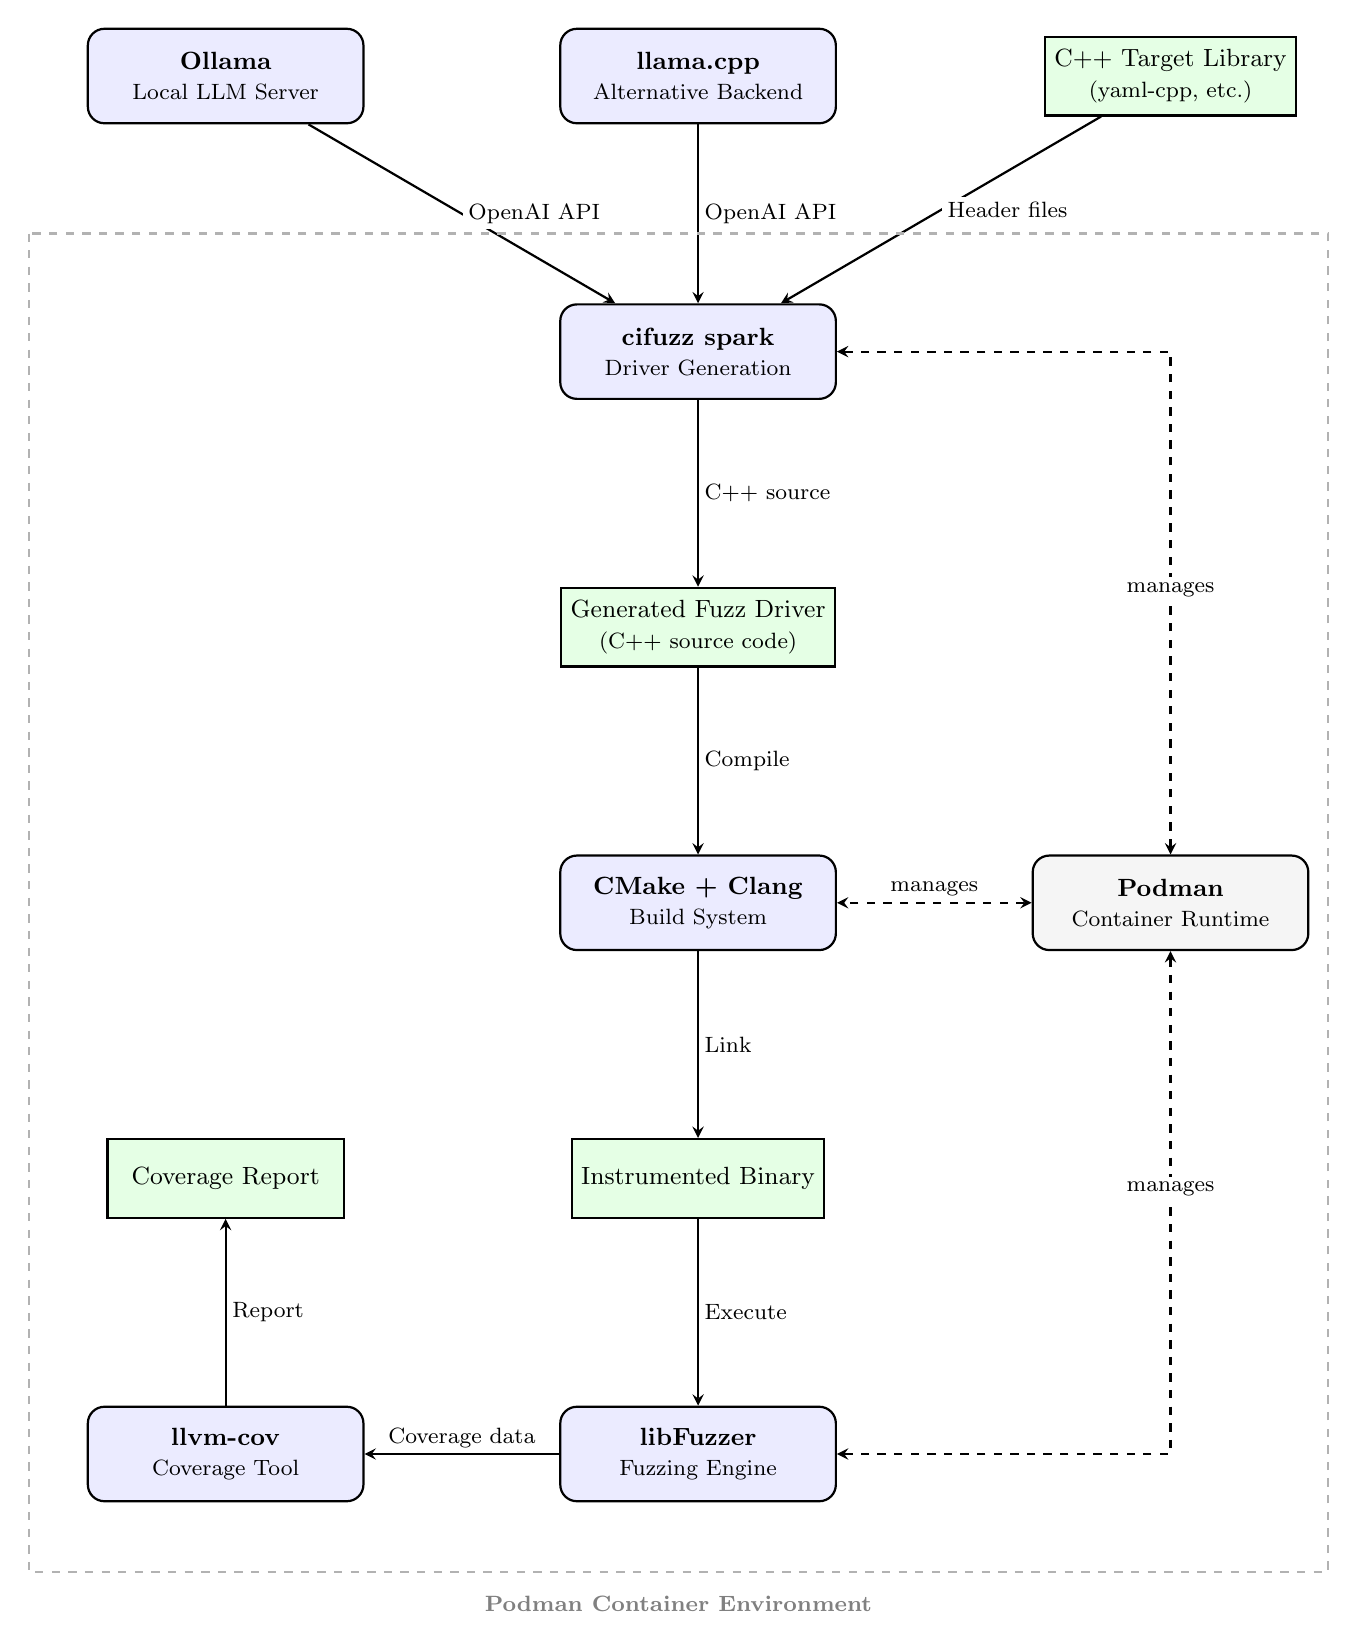
\begin{tikzpicture}[
        comp/.style={draw, rectangle, rounded corners=6pt, minimum width=3.5cm, minimum height=1.2cm, align=center, fill=blue!8, thick, font=\small},
        data/.style={draw, rectangle, minimum width=3cm, minimum height=1cm, align=center, fill=green!10, thick, font=\small},
        arrow/.style={->, >=stealth, thick},
        darrow/.style={<->, >=stealth, thick, dashed},
        elabel/.style={font=\footnotesize, fill=white, inner sep=2pt, align=center}
    ]

    % --- Row 1: LLM Servers + Target Library ---
    \node[comp] (ollama) at (0, 0) {\textbf{Ollama}\\{\footnotesize Local LLM Server}};
    \node[comp] (llamacpp) at (6, 0) {\textbf{llama.cpp}\\{\footnotesize Alternative Backend}};
    \node[data] (target) at (12, 0) {C++ Target Library\\{\footnotesize(yaml-cpp, etc.)}};

    % --- Row 2: cifuzz spark ---
    \node[comp] (cifuzz) at (6, -3.5) {\textbf{cifuzz spark}\\{\footnotesize Driver Generation}};

    % --- Row 3: Generated Driver ---
    \node[data] (driver) at (6, -7) {Generated Fuzz Driver\\{\footnotesize(C++ source code)}};

    % --- Row 4: Build ---
    \node[comp] (cmake) at (6, -10.5) {\textbf{CMake + Clang}\\{\footnotesize Build System}};

    % --- Row 5: Instrumented Binary ---
    \node[data] (binary) at (6, -14) {Instrumented Binary};

    % --- Row 6: Fuzzing Engine ---
    \node[comp] (libfuzzer) at (6, -17.5) {\textbf{libFuzzer}\\{\footnotesize Fuzzing Engine}};

    % --- Row 7: Coverage Measurement ---
    \node[comp] (llvmcov) at (0, -17.5) {\textbf{llvm-cov}\\{\footnotesize Coverage Tool}};
    \node[data] (coverage) at (0, -14) {Coverage Report};

    % --- Podman container runtime label ---
    \node[comp, fill=gray!8] (podman) at (12, -10.5) {\textbf{Podman}\\{\footnotesize Container Runtime}};

    % --- Arrows (top-down flow) ---
    \draw[arrow] (ollama) -- node[elabel, right, pos=0.5]{OpenAI API} (cifuzz);
    \draw[arrow] (llamacpp) -- node[elabel, right, pos=0.5]{OpenAI API} (cifuzz);
    \draw[arrow] (target) -- node[elabel, right, pos=0.5]{Header files} (cifuzz);
    \draw[arrow] (cifuzz) -- node[elabel, right]{C++ source} (driver);
    \draw[arrow] (driver) -- node[elabel, right]{Compile} (cmake);
    \draw[arrow] (cmake) -- node[elabel, right]{Link} (binary);
    \draw[arrow] (binary) -- node[elabel, right]{Execute} (libfuzzer);
    \draw[arrow] (libfuzzer) -- node[elabel, above]{Coverage data} (llvmcov);
    \draw[arrow] (llvmcov) -- node[elabel, right]{Report} (coverage);

    % --- Podman manages ---
    \draw[darrow] (podman) -- node[elabel, above]{manages} (cmake);
    \draw[darrow] (podman) |- node[elabel, pos=0.25, above]{manages} (libfuzzer);
    \draw[darrow] (podman) |- node[elabel, pos=0.25, above]{manages} (cifuzz);

    % Container boundary
    \draw[dashed, thick, gray!60] (-2.5, -2) rectangle (14, -19);
    \node[font=\footnotesize\bfseries, gray] at (5.75, -19.4) {Podman Container Environment};

    \end{tikzpicture}
    }
    \caption{Evaluation Environment Component Diagram. Components (rounded boxes) interact via defined interfaces. Ollama or llama.cpp serve the LLM; cifuzz spark orchestrates driver generation; CMake/Clang builds the driver; libFuzzer executes it; llvm-cov measures coverage. All build and fuzzing components run inside a Podman container. The top-down flow shows the data transformation pipeline from source code to coverage report.}
    \label{fig:eval_environment}
\end{figure}

A full evaluation cycle for one model on one target took approximately 10 to 45 minutes, depending on model size and token generation speed (see Table~\ref{tab:model_performance} in Chapter~5 for detailed timings). With 14 models and 6 primary targets, plus five runs per configuration for consistency checking, the complete Phase 1 evaluation required approximately two weeks of continuous testing.

The general fuzzing workflow (as introduced in earlier chapters) forms the foundation of our evaluation methodology, from defining targets from source code, generating fuzz tests via LLM, executing them through the fuzzing engine (libFuzzer with sanitizers), detecting crashes, and either reporting findings or mutating inputs for continued testing. Each evaluation cycle involved generating a driver, checking compilation, running the fuzzer for 60 seconds, measuring coverage with llvm-cov, and storing results.

\section{Phase 2: Model Optimization with LoRA Fine-Tuning}
\label{sec:impl_phase2}

After the initial evaluation showed promising results from Qwen 2.5-Coder models, we investigated whether fine-tuning could improve performance further. This phase addresses the optimization aspect of \textbf{RQ2}, asking whether smaller, fine-tuned models can outperform larger general-purpose models. The goal was to see if a small model, specifically trained for fuzz driver generation, could match or exceed larger ones.

\subsection{Training Data Preparation}

Most important for fine-tuning is the training data. High-quality examples of fuzz drivers paired with source code were essential. Previous work on LLM-based fuzzing like LLM4Fuzz \cite{llm4fuzz} and TitanFuzz \cite{TitanFuzz2022} has demonstrated that quality training data directly impacts generation success.

To build our dataset, we extracted training examples from OSS-Fuzz \cite{OSSFuzzBugs2021}. Google has fuzz-tested hundreds of open-source projects through OSS-Fuzz, and the fuzz drivers are publicly available. We focused on C and C++ drivers because those matched our target domain.

It is important to note that Google also maintains OSS-Fuzz-Gen~\cite{ossfuzzgen}, an automated system that uses LLMs to generate fuzz targets for OSS-Fuzz projects. While OSS-Fuzz-Gen pursues a similar high-level goal, namely automated fuzz driver creation, it differs from our approach in several important ways. OSS-Fuzz-Gen operates within Google's infrastructure, has access to complete build logs and project metadata, and targets breadth across hundreds of projects. Our approach instead focuses on depth for a specific domain (automotive C++ libraries), uses locally deployable open-source models rather than proprietary APIs, and integrates into enterprise CI/CD pipelines with strict network isolation requirements. We used OSS-Fuzz as a \emph{training data source} for fine-tuning, not as a competing tool.

Our extraction process involved four steps:

\begin{enumerate}
    \item Clone the OSS-Fuzz repository
    \item Identify projects with C/C++ fuzz drivers
    \item For each driver, extract the header files it includes
    \item Create input/output pairs: headers as input, driver as expected output
\end{enumerate}

We created two datasets:
\begin{itemize}
    \item \textbf{Small dataset}: 172 examples, focusing on quality over quantity
    \item \textbf{Extended dataset}: 709 examples, broader coverage but more noise
\end{itemize}

These examples included drivers for libraries like FreeType, LibPNG, SQLite, and zlib, covering a range of API styles from simple functions to complex object-oriented interfaces. We deliberately included diverse examples to help the model generalize rather than memorize specific patterns.

\textbf{Representativeness for automotive applications.} While these OSS-Fuzz libraries are not automotive-specific, they share key characteristics with automotive C/C++ codebases: they are written in C/C++, they expose public APIs with defined contracts, they process structured input data (configuration files, serialized data, media streams), and they must handle malformed inputs gracefully. Automotive ECU software similarly parses CAN/LIN messages, configuration files (YAML, JSON, XML), and sensor data streams. The fuzz driver patterns (consuming a byte buffer, translating it into API calls, catching exceptions) are structurally identical regardless of domain. We therefore consider these training examples representative of the \emph{structural} task of fuzz driver generation, while acknowledging that they do not capture automotive-specific safety semantics (e.g., ISO~26262 ASIL-level constraints). The OSS-Fuzz corpus remains the largest publicly available source of validated C/C++ fuzz drivers; no comparable automotive-specific corpus exists at this time.

Quality control was important. We manually reviewed a sample of the extracted drivers to verify they were functional and not stub implementations. Approximately 15\% (106 out of the initial pool) of extracted drivers were discarded because they were incomplete or contained obvious errors.

\subsection{LoRA Configuration and Training}

We used Low-Rank Adaptation (LoRA) \cite{Hu2021} rather than full fine-tuning. Full fine-tuning updates all model weights, which requires enormous compute resources. LoRA adds small trainable matrices alongside the frozen base model. This reduces memory requirements by a large margin while achieving similar results on specialized tasks.

Our LoRA configuration:

\begin{lstlisting}[language=Python, caption={LoRA Configuration Parameters}]
# LoRA Configuration
LORA_RANK = 16          # Rank controls adaptation complexity
LORA_ALPHA = 32         # Alpha is the scaling factor
DROPOUT = 0.1           # Prevents overfitting
TARGET_MODULES = ["q_proj", "v_proj", "k_proj", "o_proj"]
DEVICE = "auto"         # Uses optimal hardware
DTYPE = "float16"       # Memory-efficient precision
\end{lstlisting}

A rank of 16 was a balance between adaptation capacity and training speed. Higher ranks can capture more complex patterns but require more memory and training time. We tested ranks of 8, 16, and 32. Rank 16 produced the strongest output for our dataset size.

We trained on the Qwen 2.5-Coder 1.5B base model. This is a small model that runs quickly on modest hardware. This size was chosen to investigate whether fine-tuning could make small models competitive with larger ones.

Training used standard supervised fine-tuning:
\begin{itemize}
    \item Input: Header files and fuzzing instructions
    \item Target: Complete fuzz driver
    \item Learning rate: 2e-5 with cosine decay
    \item Epochs: 3
    \item Batch size: 4 (with gradient accumulation)
\end{itemize}

\subsection{Fine-Tuned Model Evaluation}

After training, we evaluated the fine-tuned models on the same yaml-cpp benchmark used in Phase 1. The results showed measurable efficiency improvements, summarized with absolute numbers in Table~\ref{tab:finetune_eval_impl}.

\begin{table}[htbp]
\centering
\caption{Fine-Tuned Model Evaluation Results on yaml-cpp (Absolute Numbers)}
\label{tab:finetune_eval_impl}
\small
\begin{tabular}{lcccc}
\toprule
Model Version & Gen.\ Time & Tokens Used & Time Saved & Tokens Saved \\
\midrule
Base Qwen 2.5-Coder 1.5B & 15\,min & 112\,k & (baseline) & (baseline) \\
LoRA (172 examples) & 12\,min & 65\,k & 3\,min (20\%) & 47\,k (42\%) \\
LoRA (709 examples) & 10\,min & 50\,k & 5\,min (33\%) & 62\,k (55\%) \\
\midrule
Qwen 2.5-Coder 32B (ref.) & 33\,min & 45\,k & (reference) & (reference) \\
\bottomrule
\end{tabular}
\end{table}

Coverage of the fine-tuned 1.5B models remained comparable to the larger Qwen~2.5-Coder~32B model, which achieved 43\% line coverage (see Chapter~5 for detailed coverage results). The reference row shows that while the 32B model achieves higher coverage, it requires over three times the generation time.

Fine-tuned models generated more concise code. They learned the structure of fuzz drivers and did not waste tokens on unnecessary explanations or boilerplate. These efficiency gains meant that generating each driver took less time and fewer API tokens, which directly impacts operational costs.

More training data did not always produce proportionally better results. The 709-example dataset achieved the best efficiency improvements (see Chapter~5 for detailed metrics), but it included some lower-quality drivers that may have introduced noise. While the extended dataset reduced generation time and token usage, the coverage quality did not improve proportionally. Quality matters more than quantity for fine-tuning specialized tasks.

We also tested the fine-tuned models on RapidJSON and pugixml to check generalization. Performance was similar to yaml-cpp, suggesting the fine-tuning improved general fuzz driver generation rather than overfitting to specific libraries.

\section{Phase 3: Enterprise CI/CD Integration}
\label{sec:impl_phase3}

Phase 3 focused on deploying the validated approach from Phases 1 and 2 into CARIAD's production CI/CD infrastructure using Azure OpenAI \cite{azure_openai} as the LLM backend. The central question for this phase was \textbf{RQ3}: Can LLM-assisted fuzz driver generation be integrated into secure enterprise CI/CD pipelines while meeting performance, cost, and security requirements? The transition from controlled local experiments with Ollama \cite{ollama} to enterprise deployment revealed additional infrastructure considerations that constituted the primary engineering focus of this phase.

To guide the integration, we derived the following concrete requirements from CARIAD's operational context:

\begin{itemize}
    \item \textbf{Performance requirements:}
    \begin{enumerate}
        \item Driver generation must complete within the CI/CD feedback window (targeted at 15 to 30 minutes, with up to 45 minutes acceptable for complex libraries).
        \item Fuzzing execution must not block the main build pipeline; it may run asynchronously.
        \item The system must support at least 10 target libraries per day without manual intervention.
    \end{enumerate}
    \item \textbf{Cost requirements:}
    \begin{enumerate}
        \item Annual infrastructure cost must remain below \euro{}2,000 for moderate usage.
        \item The solution must not require dedicated GPU hardware on the CI/CD runners.
        \item Token consumption must be predictable and auditable.
    \end{enumerate}
    \item \textbf{Security requirements:}
    \begin{enumerate}
        \item No proprietary source code may leave the corporate network perimeter via unencrypted or unapproved channels.
        \item LLM API access must comply with the corporate zero-trust network model.
        \item Generated code must be sandboxed (containerized) and instrumented with sanitizers before execution.
        \item API credentials must be stored in approved secret management systems (GitHub Actions secrets).
    \end{enumerate}
\end{itemize}

The architectural challenges described below arose directly from these requirements, and the solutions we developed were evaluated against them.

\subsection{Architectural Challenges}

Our initial integration strategy appeared simple in concept. The working local pipeline used standard Linux tools, and enterprise runners operated in similar environments. However, the enterprise network security policies required careful architectural planning to maintain compliance.

\textbf{Challenge 1: Network Isolation}

CARIAD operates with a zero-trust security model. CI/CD runners are isolated from the public internet, and external connections require explicit approval. Integrating cloud-based AI services within this security framework required a tailored architectural approach.

Our initial pipeline configuration was designed for direct connectivity and was subsequently adapted for the network isolation requirements. The Azure OpenAI requests were routed through the corporate firewall, which, as expected in a zero-trust environment, did not permit direct external API access.

\textbf{Important clarification regarding data sent to Azure OpenAI.} The prompts sent to the LLM contain only \emph{public header files} (function signatures, type definitions, class declarations) extracted by cifuzz spark, combined with generic fuzzing instructions. They do \emph{not} contain proprietary source code implementations, business logic, or internal documentation. The header files describe the public API surface of the target library, which is equivalent to information already visible in publicly distributed SDK packages. For open-source libraries like yaml-cpp, this information is entirely public. For internal CARIAD libraries, only the public interface declarations are transmitted, not the implementation files. This distinction was a key factor in the security review that approved the architecture.

The resulting error message required investigation to diagnose:
\begin{lstlisting}
Error: fatal: unable to access 'https://git.hub.vwgroup.com/...': 
Failed to connect to 127.0.0.1 port 9000 after 0 ms: Couldn't connect to server
\end{lstlisting}

Investigation revealed that the proxy configuration scope needed refinement to separate Azure-bound traffic from internal Git operations. The runner was directing Git traffic through the Azure proxy endpoint, which was configured exclusively for LLM API access.

\textbf{Challenge 2: Container Networking and Security Model}

Runners use Buildah containers for isolation. Each build step runs in its own network namespace, providing strong security boundaries. External service access must be explicitly configured at the container level.

\textbf{Attack model.} The container isolation addresses two distinct threat categories. First, \emph{tenant isolation}: in a shared runner environment, containers prevent one CI/CD job from accessing another's data or network connections. Buildah's rootless, daemonless architecture strengthens this boundary compared to Docker, as there is no long-running daemon with elevated privileges that could be exploited. Second, \emph{generated code containment}: since LLM-generated fuzz drivers are untrusted code, they execute inside containers with restricted privileges, no shell access, and sanitizer instrumentation (ASan/UBSan) that terminates on memory violations.

However, container isolation does \emph{not} protect against a compromised cloud provider. If the Azure infrastructure itself were malicious, it could inspect the prompts and responses. This is a fundamental limitation of any cloud-based approach and is mitigated through contractual and compliance mechanisms (Azure's SOC~2, ISO~27001, and GDPR certifications) rather than technical isolation alone. For organizations requiring protection against cloud-provider-level threats, the alternative is on-premises model deployment, which we evaluated in Phase~1 using Ollama (Section~\ref{sec:impl_phase1}).

We tried several approaches:

Host network mode:
\begin{lstlisting}[language=bash]
buildah run --network host -v $(pwd):/project $containerid /bin/bash -c "cifuzz spark target"
\end{lstlisting}
This provided the container with host-level network access, though the firewall policy continued to govern external connections.

Custom DNS entries:
\begin{lstlisting}[language=bash]
buildah run --add-host ny4mdomain.openai.azure.com:${OPENAI_IP} ...
\end{lstlisting}
This approach was not effective because the connectivity requirement originated from firewall policy rather than DNS resolution.

\textbf{Challenge 3: Credential Management}

Even with network connectivity established, API keys needed to be securely passed to the container. GitHub Actions secrets provided the storage, but injecting them into Buildah containers required explicit environment variable passing:

\begin{lstlisting}[language=bash]
buildah run \
  --env CIFUZZ_LLM_API_URL \
  --env CIFUZZ_LLM_AZURE_DEPLOYMENT_NAME \
  --env CIFUZZ_LLM_MAX_TOKENS \
  --env CIFUZZ_LLM_API_TOKEN \
  -v $(pwd):/$PROJECT_FOLDER ${{ env.containerid }} \
  /usr/bin/bash -c "cd /project/build && cifuzz spark target_name"
\end{lstlisting}

Each environment variable had to be passed explicitly. Careful validation of the configuration was necessary, as missing LLM credentials would cause the generation step to be skipped without halting the pipeline. We addressed this by adding pre-flight checks to verify all required variables before the LLM call.

\subsection{Self-Hosted Runner Solution}

Following our investigation, we determined that direct Azure OpenAI access required a network architecture aligned with the enterprise security model. We collaborated with the infrastructure team to implement an appropriate solution.

\textbf{Azure Private Link Architecture}

Our approved solution used Azure Private Link \cite{azure_private_link}. This creates a private endpoint for Azure services that appears inside the corporate network. Traffic to the LLM endpoint never crosses the public internet.

From the runner's perspective, the Azure OpenAI endpoint has an internal IP address. The firewall allows internal traffic, so the LLM calls succeed.

\textbf{Azure trust within the zero-trust model.} A natural question arises: if CARIAD operates a zero-trust network, why is Azure considered trusted? The answer is that zero-trust refers to the \emph{network perimeter}: no device or connection is trusted by default based solely on network location. Azure Private Link integrates Azure services into the corporate network as a \emph{private endpoint}, meaning the traffic never traverses the public internet and is subject to the same network security group rules as internal services. Trust in Azure as a \emph{service provider} is established through a separate mechanism: contractual agreements (Microsoft Enterprise Agreement), compliance certifications (SOC~2 Type~II, ISO~27001, C5), and data processing agreements under GDPR. The zero-trust model governs network access paths; provider trust is established through governance and compliance frameworks. This layered approach, combining a private network path with contractual trust, satisfies CARIAD's security requirements without contradicting the zero-trust principle.

Setting up Private Link involved coordination with the infrastructure team, following the organization's established approval workflow:

\begin{enumerate}
    \item Request submission with business justification
    \item Security review of the use case
    \item Azure subscription configuration
    \item DNS updates for private endpoint resolution
    \item Network security group rules
    \item Testing and validation
\end{enumerate}

We prepared a detailed business case including cost analysis (approximately \euro{}74 to \euro{}1,452 annually depending on usage) and security risk assessment. This documentation supported the approval process.

\textbf{Working Pipeline Configuration}

Once Private Link was operational, the pipeline worked reliably. Figure~\ref{fig:cicd_workflow} illustrates the CI/CD pipeline as a workflow diagram. The full YAML configuration is provided in Appendix~\ref{sec:appendix_pipeline}.

\begin{figure}[htbp]
    \centering
    \resizebox{\textwidth}{!}{
    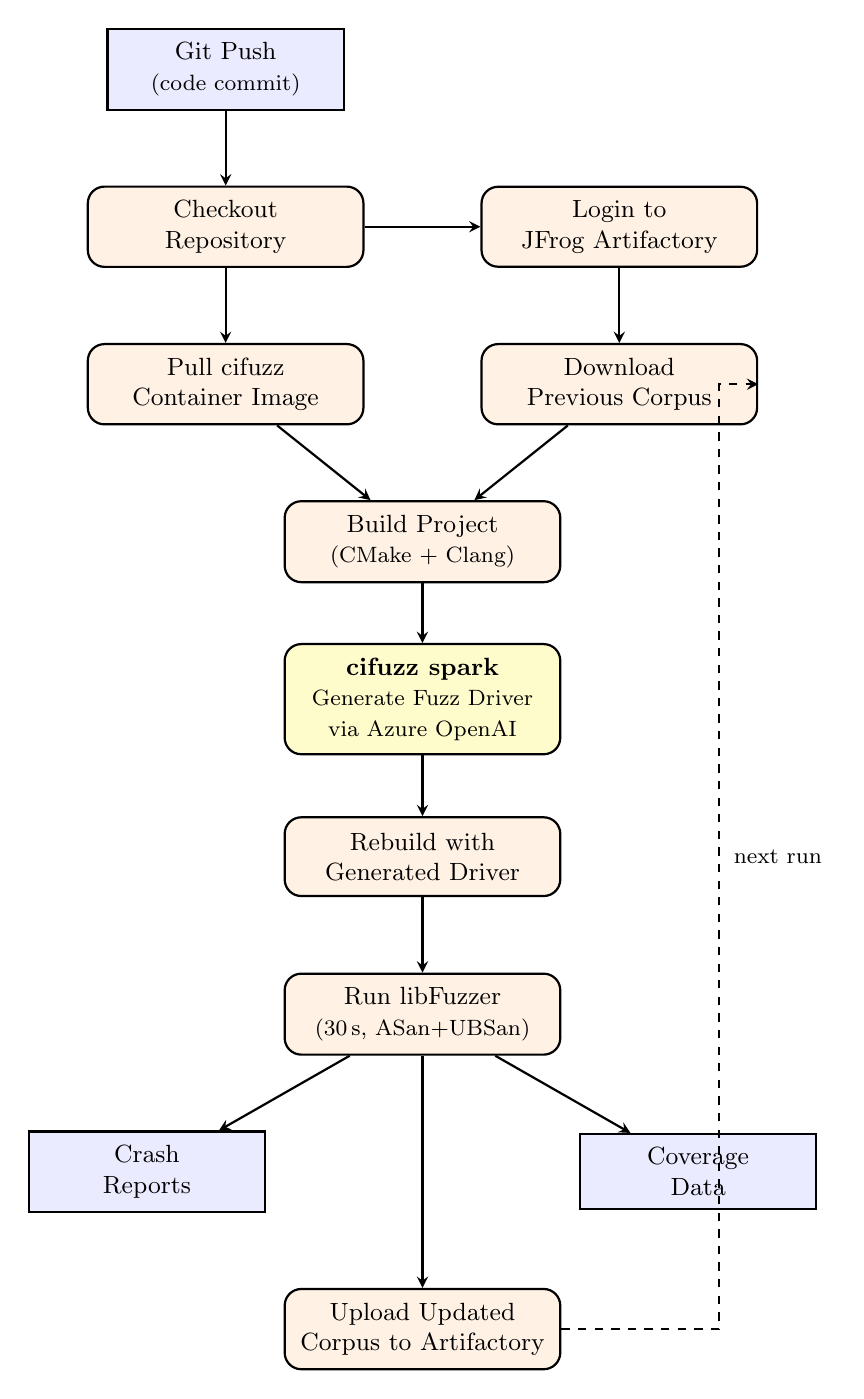
\begin{tikzpicture}[
        procstep/.style={draw, rounded corners=6pt, rectangle, minimum width=3.5cm, minimum height=1cm, align=center, fill=orange!10, thick, font=\small},
        data/.style={draw, rectangle, minimum width=3cm, minimum height=0.8cm, align=center, fill=blue!8, thick, font=\small},
        decision/.style={draw, diamond, aspect=2, minimum width=2cm, align=center, fill=yellow!15, thick, font=\small},
        arrow/.style={->, >=stealth, thick},
        every node/.style={inner sep=5pt}
    ]
    % --- Trigger ---
    \node[data] (trigger) at (0, 0) {Git Push\\{\footnotesize(code commit)}};

    % --- Row 1 ---
    \node[procstep] (checkout) at (0, -2) {Checkout\\Repository};
    \node[procstep] (login) at (5, -2) {Login to\\JFrog Artifactory};

    % --- Row 2 ---
    \node[procstep] (corpus) at (5, -4) {Download\\Previous Corpus};
    \node[procstep] (container) at (0, -4) {Pull cifuzz\\Container Image};

    % --- Row 3 ---
    \node[procstep] (build) at (2.5, -6) {Build Project\\{\footnotesize(CMake + Clang)}};

    % --- Row 4: LLM ---
    \node[procstep, fill=yellow!20] (spark) at (2.5, -8) {\textbf{cifuzz spark}\\{\footnotesize Generate Fuzz Driver}\\{\footnotesize via Azure OpenAI}};

    % --- Row 5 ---
    \node[procstep] (rebuild) at (2.5, -10) {Rebuild with\\Generated Driver};

    % --- Row 6 ---
    \node[procstep] (fuzz) at (2.5, -12) {Run libFuzzer\\{\footnotesize(30\,s, ASan+UBSan)}};

    % --- Row 7: outputs ---
    \node[data] (crashes) at (-1, -14) {Crash\\Reports};
    \node[data] (coverage) at (6, -14) {Coverage\\Data};

    % --- Row 8 ---
    \node[procstep] (upload) at (2.5, -16) {Upload Updated\\Corpus to Artifactory};

    % --- Arrows ---
    \draw[arrow] (trigger) -- (checkout);
    \draw[arrow] (checkout) -- (login);
    \draw[arrow] (login) -- (corpus);
    \draw[arrow] (checkout) -- (container);
    \draw[arrow] (container) -- (build);
    \draw[arrow] (corpus) -- (build);
    \draw[arrow] (build) -- (spark);
    \draw[arrow] (spark) -- (rebuild);
    \draw[arrow] (rebuild) -- (fuzz);
    \draw[arrow] (fuzz) -- (crashes);
    \draw[arrow] (fuzz) -- (coverage);
    \draw[arrow] (fuzz) -- (upload);

    % --- Feedback ---
    \draw[arrow, dashed] (upload.east) -- ++(2,0) |- node[right, pos=0.25, font=\footnotesize]{next run} (corpus.east);

    \end{tikzpicture}
    }
    \caption{CI/CD Pipeline Workflow. Processing steps are in rounded boxes; data artifacts in rectangular boxes. The highlighted step (cifuzz spark) invokes the LLM via Azure Private Link. Corpus persistence through JFrog Artifactory enables cumulative coverage improvement across runs.}
    \label{fig:cicd_workflow}
\end{figure}

Our pipeline includes corpus persistence through JFrog Artifactory. Each run downloads the previous corpus, runs fuzzing to extend it, and uploads the updated corpus. This way, coverage improvements accumulate over time rather than starting fresh each build.

The network architecture required for this deployment is illustrated in Figure~\ref{fig:enterprise_network} (Chapter 6). As discussed in the subsequent Discussion chapter, the Azure Private Link setup enables secure communication between the CARIAD internal network and Azure OpenAI services without routing traffic through the public internet, while maintaining full security compliance. This architectural solution was the key component for enterprise deployment.

\subsection{Operational Considerations}

With the technical implementation complete, several operational concerns remained.

\textbf{Cost Management}

Azure OpenAI charges per token. Each fuzz driver generation uses approximately 3000 to 8000 tokens depending on the target complexity. We calculated costs for different usage scenarios:

\begin{table}[htbp]
\centering
\caption{Azure OpenAI Cost Projections for Different Usage Scenarios}
\label{tab:cost_scenarios_impl}
\small
\begin{tabular}{lcccc}
\toprule
Scenario & Targets/Day & Builds/Day & Annual Tokens & Annual Cost \\
\midrule
Light & 5 & 1 & 3.1M & \euro{}74 \\
Moderate & 10 & 2 & 12.5M & \euro{}219 \\
Heavy & 25 & 5 & 78M & \euro{}726 \\
Enterprise & 50 & 10 & 156M & \euro{}1,452 \\
\bottomrule
\end{tabular}
\end{table}

These costs are low in absolute terms. For context, even the enterprise usage scenario represents a modest investment compared to manual security testing efforts. However, the LLM-generated drivers supplement rather than replace expert security engineering work, so this comparison captures only the infrastructure cost component. A detailed economic analysis including human oversight costs appears in Chapter~5.

\textbf{Failure Handling}

LLM outputs are non-deterministic. Sometimes the generated driver does not compile. Sometimes it compiles but crashes immediately. The pipeline was designed to handle these cases gracefully.

We added fallback logic, so if the LLM-generated driver fails, the pipeline falls back to any existing manually-written drivers. The build does not fail due to unsuccessful AI generation. Generated drivers that work are kept. Those that fail are logged for review but do not block the pipeline.

\textbf{Security Review}

Generated code running in CI/CD pipelines poses security considerations. What if the LLM generates malicious code? We addressed this concern in our security review:

\begin{enumerate}
    \item The code runs inside containers with limited privileges
    \item ASan and UBSan catch memory-related errors and undefined behavior during execution
    \item Generated code is compiled and executed, not given shell access
    \item The LLM only sees public header files, not sensitive source code
    \item All generated code is logged for audit purposes
\end{enumerate}

After reviewing these controls, the security team approved the architecture. They requested additional monitoring of token usage and periodic audits of generated code quality.

The next chapter presents experimental results in detail, with quantitative analysis of model performance and coverage metrics across all evaluated configurations.